\documentclass[11pt, oneside]{article} 
\usepackage{geometry}
\geometry{letterpaper} 
\usepackage{graphicx}
	
\usepackage{amssymb}
\usepackage{amsmath}
\usepackage{parskip}
\usepackage{color}
\usepackage{hyperref}

\graphicspath{{/Users/telliott_admin/Dropbox/Tex/png/}}
% \begin{center} 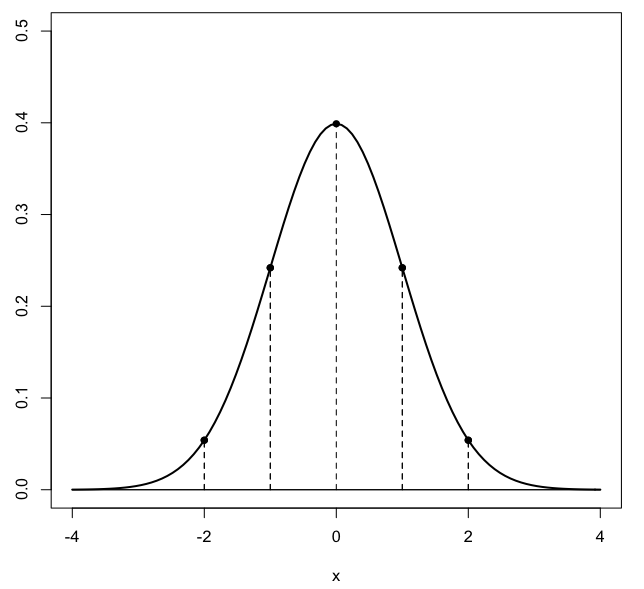
\includegraphics [scale=0.4] {gauss3.png} \end{center}

\title{Quick review}
\date{}

\begin{document}
\maketitle
\Large
We do a quick review with differentiation of basic complex functions of $z$:  $z$, $z^2$, $\sqrt{z}$, $1/z$, Log$(z)$, $e^z$, $\cos z$, and $\sin z$.
\subsection*{z}
\[ z = x + iy = u(x,y) + iv(x,y) \]
\[ u_x = 1 = v_y \]
\[ u_y = 0 = v_x \]
I guess this qualifies as meeting CRE.
\[ (z)' = u_x + i v_x = 1 \]
Note:  for $\bar{x} = x* = x - iy$, $u_x \ne v_y$ and CRE are \emph{not} satisfied.

\subsection*{z$^2$}
\[ z^2 = (x + iy)(x + iy) = x^2 - y^2 + i2xy \]
\[ u_x = 2x = v_y \]
\[ u_y = -2y = - v_x \]
\[ (z^2)' = u_x + i v_x = 2x + i 2y = 2 z \]

\subsection*{$\sqrt{z}$}
This one is easiest in polar coordinates.  Take the principal value:
\[ f(z) = \sqrt{z} = \sqrt{r} e^{i \theta/2} \]

We need to rewrite this as $z = u(r,\theta) + i v(r, \theta)$
\[ u(r,\theta) = \sqrt{r} \cos \theta/2 \]
\[ v(r,\theta) = \sqrt{r} \sin \theta/2 \]
So
\[ u_r = \frac{1}{2 \sqrt{r}} \cos \theta/2 \]
\[ u_{\theta} = \sqrt{r} \ \frac{1}{2} \  (- \sin \theta/2) \]
\[ v_r = \frac{1}{2 \sqrt{r}} \sin \theta/2 \]
\[ v_{\theta} = \sqrt{r} \ \frac{1}{2} \  \cos \theta/2 \]

We see that
\[ r u_r = v_{\theta} \]
\[ r v_r = - u_{\theta} \]
The polar CRE are satisfied and
\[ (\sqrt{z})' = e^{-i\theta} (u_r + i v_r) \]
\[ = e^{-i\theta} (\frac{1}{2 \sqrt{r}} \cos \theta/2 + i \frac{1}{2 \sqrt{r}} \sin \theta/2 \]
\[ = e^{-i\theta} \frac{1}{2 \sqrt{r}} e^{i \theta/2} =  \frac{1}{2 \sqrt{r}} e^{- i \theta/2} \]
\[ = \frac{1}{2 \sqrt{z}} \]

For an explanation of where that $e^{-i\theta}$ comes from in the polar form of the derivative, see the chapter on the polar CRE in our write-up on complex analysis.

\subsection*{1/z}
\[ \frac{1}{z} = \frac{1}{x + iy} = \frac{x - iy}{(x + iy)(x - iy)} = \frac{x - iy}{x^2 + y^2} \]
Every partial derivative will have a factor of $(x^2 + y^2)^2$ in the denominator.  It is easier if we just remember that and don't write it explicitly:\
\[ u_x = x^2 + y^2 - 2x^2 = y^2 - x^2 \]
\[ u_y = -2xy \]
\[ v_x = 2xy \]
\[ v_y = x^2 + y^2 - 2y^2 = y^2 - x^2 \]So
So $u_x = v_y$ and $u_y = -v_x$ and CRE are satisfied.
\[ \ [ \ \frac{1}{z} \ ]' = u_x + i v_x =  \frac{y^2 - x^2}{(x^2 + y^2)^2} + i \ \frac{2xy}{(x^2 + y^2)^2} \]
We feel that this derivative should be equal to $-1/z^2$.  So let's try to work backward, leaving the minus sign out for now.
\[ \frac{1}{z^2} = \frac{1}{z} \ \frac{1}{z} = \frac{z*}{zz*} \ \frac{z*}{zz*} \]
So the denominator is clearly correct.
\[ (zz*)^2 = (x^2 + y^2)^2 \]
On top we have
\[ (z*)^2 = (x - iy)(x - iy) = x^2 - y^2 -i2xy \]
???
But remember the minus sign, we really have
\[ (z*)^2 = y^2 - x^2 + i2xy \]
This matches what we have from $u_x + i v_x$.
\[ [ \ \frac{1}{z} \ ]' = - \frac{1}{z^2} \]

\subsection*{1/z in polar form}
****

\subsection*{Log(z)}
\[ \text{Log}(z) = \text{Log}(r e^{i \theta}) = \ln r + i \theta \]
Now rewrite in terms of $x$ and $y$:
\[ = \ln \sqrt{x^2 + y^2} + i \tan^{-1} \frac{y}{x} \]
\[ = \frac{1}{2} \ln x^2 + y^2 + i \tan^{-1} \frac{y}{x} \]
\[ u_x = \frac{1}{2}  \frac{1}{(x^2 + y^2)} \ 2x = \frac{x}{x^2 + y^2} \]
\[ u_y = \frac{y}{x^2 + y^2} \]
\[ v_x = \frac{1}{1 + (y/x)^2)} \ (-\frac{y}{x^2}) = -\frac{y}{x^2 + y^2}  \]
\[ v_y = \frac{1}{1 + (y/x)^2)} \ {1/x} = \frac{x}{x^2 + y^2} \]
So $u_x = v_y$ and $u_y = -v_x$ and CRE are satisfied.
\[ \ [ \ \text{Log}(z) \ ]' = u_x + i v_x = \frac{x}{x^2 + y^2} - i \frac{y}{x^2 + y^2}  \]
\[ = \frac{z*}{z z*} = \frac{1}{z} \]

\subsection*{exp(z)}
\[ e^z = e^{x + iy} = e^x \ e^{iy} = e^x (\cos y + i \sin y) \]
\[ = e^x \cos y + ie^x \ \sin y \]
\[ u_x = e^x \cos y \]
\[ u_y = - e^x \sin y \]
\[ v_x = e^x \sin y \]
\[ v_y = e^x \cos y \]
So $u_x = v_y$ and $u_y = -v_x$ and CRE are satisfied.
\[ (e^z)' = e^x \cos y + i e^x \sin y = e^z \]

\subsection*{cos z and sin z}
To begin, we suppose that Euler's formula also works for complex numbers
\[ e^{iz} = \cos z + i \sin z \]
\[ e^{-iz} = \cos z - i \sin z \]
then
\[ \cos z = \frac{1}{2} \ [ \ e^{iz} + e^{-iz} \ ] \] 
\[ \sin z = \frac{1}{2i} \ [ \ e^{iz} - e^{-iz} \ ] \] 
We can take derivatives with respect to $z$ easily:
\[ (\cos z)' = \frac{1}{2} \ [ \ i e^{iz} - i e^{-iz} \ ] \] 
\[ = - \frac{1}{2i} \ [ \ e^{iz} - e^{-iz} \ ] = - \sin z \] 

\[ (\sin z)' = \frac{1}{2i} \ [ \ ie^{iz} + ie^{-iz} \ ] \] 
\[ = \frac{1}{2} \ [ \ e^{iz} + e^{-iz} \ ] = \cos z \] 

There is another way to get this result which separates $z$ into $u(x,y)$ and $v(x,y)$.

We need a preliminary result, consider a purely imaginary $z$:
\[ z = iy \]
Then
\[ e^{iz} = e^{iiy} = e^{-y}  \]
\[ e^{-iz} = e^{-iiy} = e^{y} \]
\[ \cos iy = \frac{1}{2} \ [ \ e^{iz} + e^{-iz} \ ] = \frac{1}{2} \ [ \ e^{-y} + e^{y} \ ] \]
The term on the right may be familiar from calculus, it is $\cosh y$.
\[ \cos iy = \cosh y \]
Similarly
\[ \sin iy = \frac{1}{2i} \ [ \ e^{iz} - e^{-iz} \ ] = \frac{1}{2i} \ [ \ e^{-y} - e^{y} \ ] \]
Having $i$ on the bottom is the same as $-i$ on the top.  We use the factor of -1 to switch the order of terms:
\[ \sin iy = i \frac{1}{2} \ [ \ e^{y} - e^{-y} \ ]  = i \sinh y \]

Now we proceed with the cosine first
\[ \cos z = \cos x + iy \]
\[ = \cos x \cos iy - \sin x \sin iy \]
\[ = \cos x \cosh y - i \sin x \sinh y \]

For the sine:
\[ \sin z = \sin x + iy \]
\[ = \sin x \cos iy + \cos x \sin iy \]
\[ = \sin x \cosh y + i \cos x \sinh y \]

Note that we have separated $u(x,y)$ from $v(x,y)$.  This allows us to test the CRE, cosine first.

Note that $\sinh y' = \cosh y$ and $\cosh y' = \sinh y$ so
\[ u_x = -\sin x \cosh y \]
\[ u_y = \cos x \sinh y \]
\[ v_x = - \cos x \sinh y \]
\[ v_y = - \sin x \cosh y \]
So $u_x = v_y$ and $u_y = -v_x$ and the CRE are satisfied.

Write the derivative.
\[ \ [ \cos z \ ]' = u_x + i v_x = - \sin x \cosh y - i \cos x \sinh y = - \sin z   \]

For the sine:
\[ u_x = \cos x \cosh y \]
\[ u_y = \sin x \sinh y \]
\[ v_x = - \sin x \sinh y \]
\[ v_y = \cos x \cosh y \]
So $u_x = v_y$ and $u_y = -v_x$ and CRE are satisfied.

\[ \ [ \sin z \ ]' = u_x + i v_x = \cos x \cosh y - i \sin x \sinh y = \cos z  \]


\end{document}